\documentclass[sigconf]{acmart}

\usepackage[utf8]{inputenc}
\usepackage{booktabs} % For formal tables


% Copyright
%\setcopyright{none}
%\setcopyright{acmcopyright}
%\setcopyright{acmlicensed}
\setcopyright{rightsretained}
%\setcopyright{usgov}
%\setcopyright{usgovmixed}
%\setcopyright{cagov}
%\setcopyright{cagovmixed}


% DOI
%\acmDOI{10.475/123_4}

% ISBN
%\acmISBN{123-4567-24-567/08/06}

%Conference
\acmConference[WWW'18]{The Web Conference}{April 2018}{Lyon, France}
\acmYear{2018}
\copyrightyear{2018}


%\acmArticle{4}
%\acmPrice{15.00}

% These commands are optional
%\acmBooktitle{Transactions of the ACM Woodstock conference}
%\editor{Jennifer B. Sartor}
%\editor{Theo D'Hondt}
%\editor{Wolfgang De Meuter}

\begin{document}
\title{Learning to Recognize Musical Genre from Audio}
%\titlenote{}
\subtitle{Challenge Overview}
%\subtitlenote{}


\author{Michaël Defferrard}
\orcid{0000-0002-6028-9024}
\affiliation{%
  \institution{EPFL, Lausanne, Switzerland}
}
\email{michael.defferrard@epfl.ch}

\author{Sharada P. Mohanty}
\affiliation{%
  \institution{EPFL, Lausanne, Switzerland}
}
\email{sharada.mohanty@epfl.ch}

\author{Sean Carroll}
\affiliation{%
  \institution{EPFL, Lausanne, Switzerland}
}
\email{sean.carroll@epfl.ch}

\author{Marcel Salathé}
\affiliation{%
  \institution{EPFL, Lausanne, Switzerland}
}
\email{marcel.salathe@epfl.ch}

% The default list of authors is too long for headers.
%\renewcommand{\shortauthors}{M. Defferrard et al.}

% Content
% * show statistics (e.g. results over time for all participants)
% * discuss the challenge
% * offer an overview of the approaches that have been tried
% * paper corresponds to what we'll talk about at the conference
% * summary of what we learned overall during the challenge
% * compile the initial proposal on the challenge design into a paper
% * include stats of participation from the challenge
% * summary of our experience running the challenge
% * major problems faced
% * suggestions for future versions of the challenge

\begin{abstract}
	todo
\end{abstract}


% The code below should be generated by the tool at
% http://dl.acm.org/ccs.cfm
 \begin{CCSXML}
<ccs2012>
  <concept>
    <concept_id>10002951.10003317.10003371.10003386.10003390</concept_id>
    <concept_desc>Information systems~Music retrieval</concept_desc>
    <concept_significance>500</concept_significance>
  </concept>
  <concept>
    <concept_id>10010147.10010257.10010258.10010259</concept_id>
    <concept_desc>Computing methodologies~Supervised learning</concept_desc>
    <concept_significance>300</concept_significance>
  </concept>
</ccs2012>
\end{CCSXML}
\ccsdesc[500]{Information systems~Music retrieval}
\ccsdesc[300]{Computing methodologies~Supervised learning}

\keywords{Music Information Retrieval (MIR), Challenge, Open Data}
% Benchmarking


\maketitle

\section{Introduction}

Like never before, the web has become a place for sharing creative work --- such as music --- among a global community of artists and art lovers. While music and music collections predate the web, the web enabled much larger scale collections. Whereas people used to own a handful of vinyls or CDs, they nowadays have instant access to the whole of published musical content via online platforms such as Spotify, iTunes, Youtube, FMA, Jamendo, Bandcamp, etc. Such dramatic increase in the size of music collections created two challenges: (i) the need to automatically organize a collection (as users and publishers cannot manage them manually anymore), and (ii) the need to automatically recommend new songs to a user knowing his listening habits. An underlying task in both those challenges is to be able to group song in semantic categories.

The task of this challenge, one of the four official challenges of the Web Conference (WWW2018) challenges track, is to recognize the musical genre of a piece of music of which only a recording is available. Genres are broad, e.g.\ pop or rock, and each song only has one target genre.
% TODO: maybe remove the below.
Other metadata, e.g.\ the song title or artist name, shall not be used for the prediction. The submitted algorithms shall learn to map an audio signal, i.e.\ a time series, to one of the 16 target genres.

The data for this challenge comes from the recently published FMA dataset~\cite{fma_dataset}, which is a dump of the Free Music Archive\footnote{\url{https://freemusicarchive.org}} (FMA), an interactive library of high-quality and curated audio which is freely and openly available to the public.
That dataset is a collection of 917 GiB and 343 days of Creative Commons-licensed audio from 106,574 tracks from 16,341 artists and 14,854 albums, arranged in a hierarchical taxonomy of 161 genres. It provides full-length and high-quality audio, pre-computed features, together with track- and user-level metadata, tags, and free-form text such as biographies.

\section{Music Genre Recognition}

Music genres are categories that have arisen through a complex interplay of cultures, artists, and market forces to characterize similarities between compositions and organize music collections. Yet, the boundaries between genres still remain fuzzy, making the problem of music genre recognition (MGR) a nontrivial task~\cite{mir_review_genre}. While its utility has been debated, mostly because of its ambiguity and cultural definition, it is widely used and understood by end-users who find it useful to discuss musical categories~\cite{mgr_why}. As such, it is one of the most researched areas in the Music Information Retrieval (MIR) field.\footnote{See e.g.\ \cite{mgr_eval_1} for an extensive list of \textasciitilde500 references to works targeting MGR as of 2012.}

% TODO: maybe remove the below.
Given the extent to which MGR is studied, we can expect many groups from the MIR community to be interested. Moreover, given the well-defined scope of the challenge, we can expect members of the wider machine learning community to participate as well. Both communities are well versed in challenges, with e.g. Kaggle and NIPS for the ML community and the MIREX for the MIR community.

\section{The Challenge}

To avoid overfitting and cheating, the challenge will happen in two rounds. The final ranking will be based on results from the second round.
The training data for both rounds consisted of the FMA medium subset, which is composed of 25,000 clips of 30 seconds, categorized in 16 genres. The categorization is unbalanced with 21 to 7,103 clips per genre, but only one genre per track. As the data is public, we collected new test data for the second round to prevent access to the test set.

In the first round, participants have been provided a test set of 30,000 clips of 30 seconds each and had to submit the predicted genre for each of these clips. The platform evaluated the predictions and ranked the participants upon submission. A subset of these clips were sampled from the FMA large dataset, while ensuring that the 30 seconds window present in the final test set do not overlap with any of the 30 seconds clips provided in the training set. The other subset was sampled from songs in the FMA full dataset, which are not present in the medium subset.
%, but have at least two top genres. During evaluation, if the prediction matches any of these two top genres, then the prediction will be considered as correct.

For the second round, the participants had to wrap their models in a docker container which encapsulated the prediction code and their trained model.
%Historical data shows that around 1000 new tracks are uploaded per month. These 1000 new tracks will be sliced into numerous 30 second clips; and a final evaluation will be run using the docker containers provided at the end of the first round. The final standings at the end of this round will determine the winner(s).
We evaluated those against a new unseen test set. These 30s clips were sampled from new contributions to the Free Music Archive.
% TODO
The participants were also asked to post online the code of their approach as well as an executive summary of the method used to be eligible for the second round.

Both rounds used the same evaluation metric. The primary score was the mean log loss and the secondary score was the mean $F_1$ score.
%For the subset of the test images which can have multiple correct genres, cross entropy loss with logits will be used to contribute to the final score.
The mean log loss is defined by
\begin{equation}
	L = - \frac{1}{N} \sum_{n=1}^N \sum_{c=1}^{C} y_{nc} \ln(p_{nc}),
\end{equation}
where $N=35000$ is the number of examples in the test set,
$C=16$ is the number of class labels, i.e.\ genres,
$y_{nc}$ is a binary value indicating if the n-th instance belongs to the $c$-th label,
$p_{nc}$ is the probability according to your submission that the $n$-th instance belongs to the $c$-th label,
$\ln$ is the natural logarithmic function.
The $F_1$ score for a particular class $c$ is given by
\begin{equation}
	F_1^c = 2\frac{p^c r^c}{p^c + r^c}, \hspace{1em}
	p^c = \frac{tp^c}{tp^c + fp^c}, \hspace{1em}
	r^c = \frac{tp^c}{tp^c + fn^c},
\end{equation}
where
$p^c$ is the precision for class $c$,
$r^c$ is the recall,
$tp^c$ refers to the number of true positives,
$fp^c$ refers to the number of false positives,
$fn^c$ refers to the number of false negatives.
The final mean $F_1$ score is then defined as
\begin{equation}
	F_1 = \frac{1}{C} \sum_{c=1}^{C} F_1^c.
\end{equation}

The challenge is hosted on crowdAI, a public platform for open challenges. Instructions to participate, training and test data, graded submissions, and the leaderboard are available on the challenge page.\footnote{\url{https://www.crowdai.org/challenges/www-2018-challenge-learning-to-recognize-musical-genre}}
Moreover, we developed a starter kit\footnote{\url{https://github.com/crowdAI/crowdai-musical-genre-recognition-starter-kit}} which includes code to handle the data and make a submission. It also features some examples and a baseline.

Participants were encouraged to check out the FMA paper~\cite{fma_dataset} for a detailed description of the data as well as the github repository\footnote{\url{https://github.com/mdeff/fma}} for Jupyter notebooks showing how to use the data, exploring it, and training baseline models.\footnote{This challenge used the \texttt{rc1} version of the data.}

\section{Results}

% Statistics about the challenge (number of submissions, participants)
% Evolution of top performance (or per participant) over time
% Ranking on round 1
% Summarize the approaches taken by the two accepted papers (and cite them)

\begin{figure}[h]
\label{fig:jointplot}
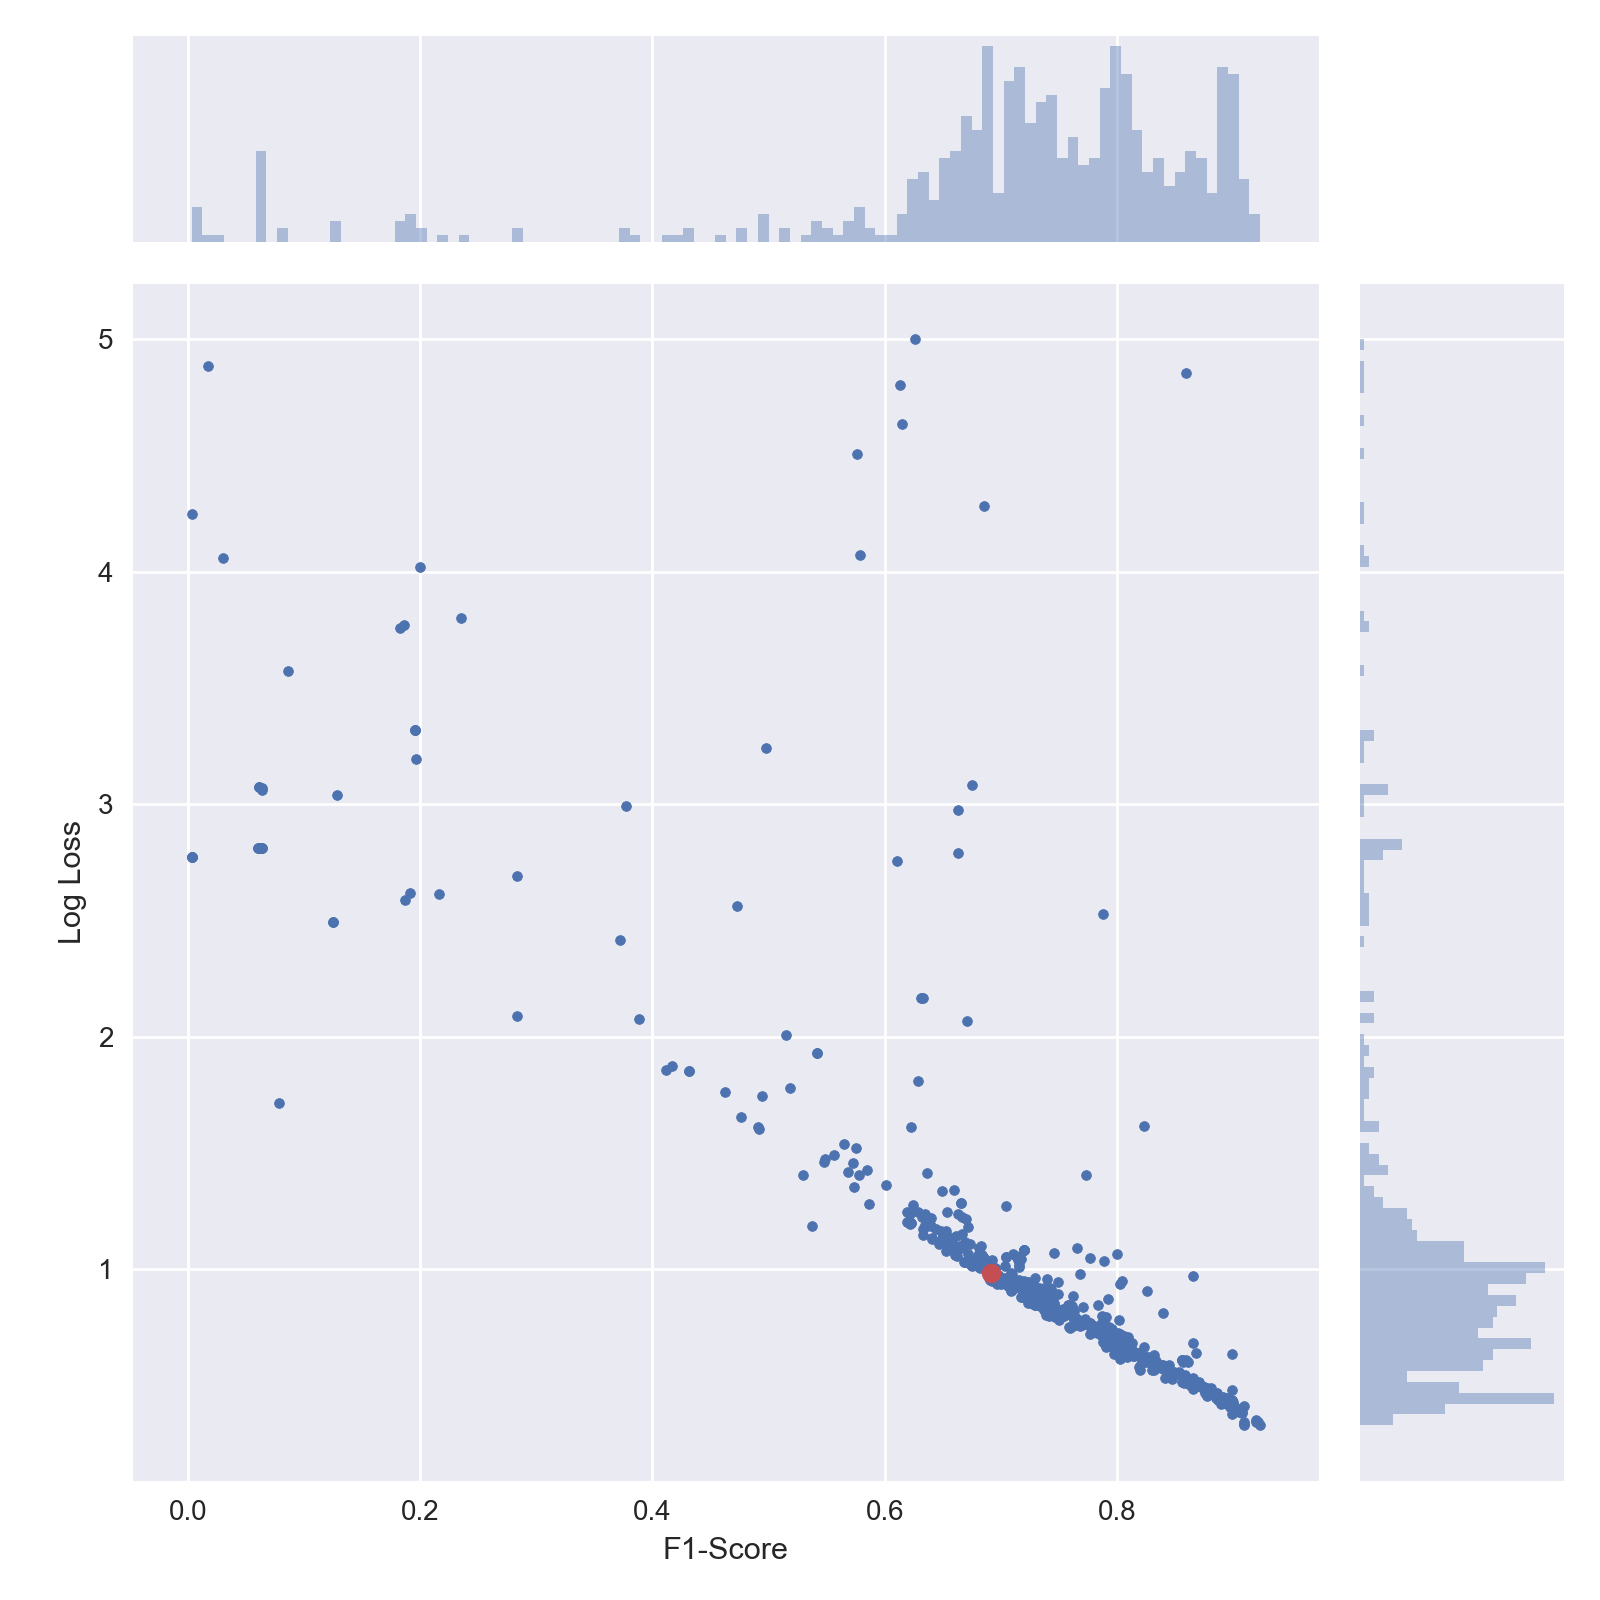
\includegraphics[width=8cm]{images/plot-1}
\centering
\caption{Joint plot of the distribution of the $F_1 score$  and the $Log Loss$ of all valid submissions made by the participants. The point marked in red represents the baseline submission prepared by the organisers at the beginning of the challenge. The plot only considers submissions with $Log Loss < 5 $ for interpretability. }
\end{figure}

At the end of the first round of the challenge, we had engaged a total of 246 participants, who either made a submission, downloaded the datasets, or contributed in the discussion forums. From these 246 participants 59 participants made atleast one submission,   with some of the top participants making as many as 110 submissions through the period of the 1st Round of the challenge. 
A total of 671 submissions were made in the first round, and of these, 77 were invalid submissions and 576 submissions were successfully graded. 
From the 576 successfully graded submissions, a total of 364 submissions had a score better than the baseline submission provided by the organisers, based on their own previous work. Figure \ref{fig:jointplot} shows the distribution of the $F_1 Score$ and the $Log Loss$ for valid submissions in the challenge.
The current rank \#1 on the leaderboard of the challenge has a $F_1 Score$ of $0.909$ and a $LogLoss$ of $0.330$, improving the state of art \textbf{(TODO: Add @michael's paper's citation)}  on this problem by \textbf{@michael: can you compute this value ?}.
Figure \ref{fig:timeline} shows the progression of scores of all the participants through the Round-1 of the challenge, with each line representing one active participant in the challenge and their top-score at the point of time referenced by the X-axis.

\begin{figure*}[h]
\label{fig:timeline}
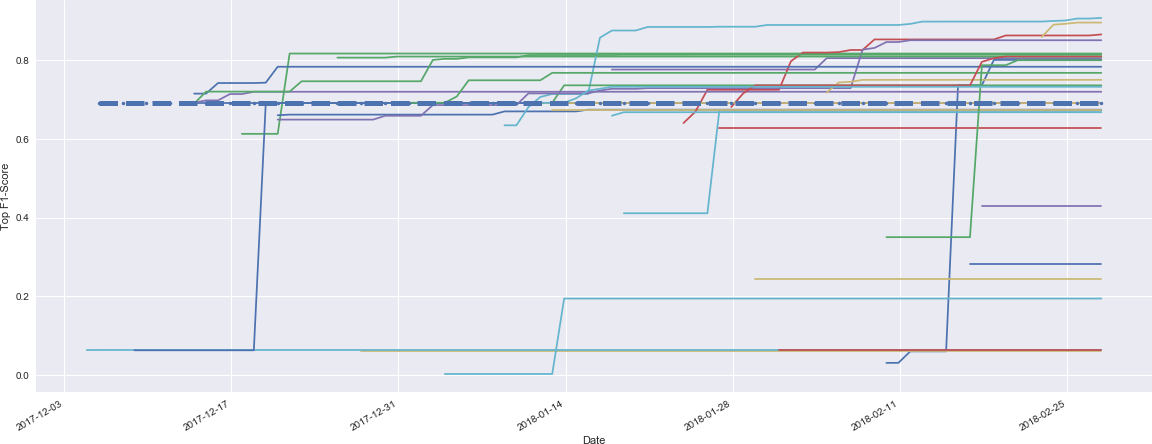
\includegraphics[width=\linewidth]{images/plot-2}
\caption{ Plot of progression of scores of all the participants through Round-1 of the challenge. Each line represents one active participant in the challenge, and their top-score at the point of time referenced by the X-axis. The dotted blue line represents the baseline score from the baseline submission.}
\end{figure*}

\section{Conclusion}

That challenge is part of an effort to promote open evaluation in machine learning for music data, which the release of the open FMA dataset was the first step~\cite{fma_dataset}. The goal of the initiative is to establish a reference benchmark based on open data. MIR research has historically suffered from the lack of publicly available benchmark datasets, which stem from the commercial interest in music by record labels, and therefore imposed rigid copyright. The FMA's solution was to aim for tracks which license permits redistribution. All data and code produced during the project and challenge are released under the CC BY 4.0 and MIT licenses.
%The release of the dataset was acclaimed online, both by scientists on Twitter and GitHub, and on the FMA blog.

% TODO: complete after round2
%\appendix
%\section{Submitted methods}
%Below is a list to all the submitted methods to the challenge.

\bibliographystyle{ACM-Reference-Format}
\bibliography{refs}

\end{document}
